%%%%%%%%%%%%%%%%%%%%%%%%%%%%%%%%%%%%%%%%%
% Beamer Presentation
% LaTeX Template
% Version 1.0 (10/11/12)
%
% This template has been downloaded from:
% http://www.LaTeXTemplates.com
%
% License:
% CC BY-NC-SA 3.0 (http://creativecommons.org/licenses/by-nc-sa/3.0/)
%
%%%%%%%%%%%%%%%%%%%%%%%%%%%%%%%%%%%%%%%%%

%----------------------------------------------------------------------------------------
%	PACKAGES AND THEMES
%----------------------------------------------------------------------------------------

\documentclass{beamer}

\mode<presentation> {

% The Beamer class comes with a number of default slide themes
% which change the colors and layouts of slides. Below this is a list
% of all the themes, uncomment each in turn to see what they look like.

%\usetheme{default}
%\usetheme{AnnArbor}
%\usetheme{Antibes}
%\usetheme{Bergen}
%\usetheme{Berkeley}
%\usetheme{Berlin}
%\usetheme{Boadilla}
%\usetheme{CambridgeUS}
%\usetheme{Copenhagen}
%\usetheme{Darmstadt}
%\usetheme{Dresden}
%\usetheme{Frankfurt}
%\usetheme{Goettingen}
%\usetheme{Hannover}
%\usetheme{Ilmenau}
%\usetheme{JuanLesPins}
%\usetheme{Luebeck}
\usetheme{Madrid}
%\usetheme{Malmoe}
%\usetheme{Marburg}
%\usetheme{Montpellier}
%\usetheme{PaloAlto}
%\usetheme{Pittsburgh}
%\usetheme{Rochester}
%\usetheme{Singapore}
%\usetheme{Szeged}
%\usetheme{Warsaw}

% As well as themes, the Beamer class has a number of color themes
% for any slide theme. Uncomment each of these in turn to see how it
% changes the colors of your current slide theme.

%\usecolortheme{albatross}
%\usecolortheme{beaver}
%\usecolortheme{beetle}
%\usecolortheme{crane}
%\usecolortheme{dolphin}
%\usecolortheme{dove}
%\usecolortheme{fly}
%\usecolortheme{lily}
%\usecolortheme{orchid}
%\usecolortheme{rose}
%\usecolortheme{seagull}
%\usecolortheme{seahorse}
%\usecolortheme{whale}
%\usecolortheme{wolverine}

%\setbeamertemplate{footline} % To remove the footer line in all slides uncomment this line
\setbeamertemplate{footline}[page number] % To replace the footer line in all slides with a simple slide count uncomment this line

\setbeamertemplate{navigation symbols}{} % To remove the navigation symbols from the bottom of all slides uncomment this line
}
\newcommand{\bftheta}{\mbox{\boldmath $\theta$}}
\newcommand{\BY}{\mbox{\boldmath $Y$}}
\newcommand{\bn}{\mbox{\boldmath $n$}}
\newcommand{\bc}{\mbox{\boldmath $c$}}
  \newcommand{\BZ}{\mbox{\boldmath $Z$}}
\usepackage{graphicx} % Allows including images
\usepackage{booktabs} % Allows the use of \toprule, \midrule and \bottomrule in tables
%\usepackage {tikz}
\usepackage{tkz-graph}
\GraphInit[vstyle = Shade]
\tikzset{
  LabelStyle/.style = { rectangle, rounded corners, draw,
                        minimum width = 2em, fill = yellow!50,
                        text = red, font = \bfseries },
  VertexStyle/.append style = { inner sep=5pt,
                                font = \normalsize\bfseries},
  EdgeStyle/.append style = {->, bend left} }
\usetikzlibrary {positioning}
%\usepackage {xcolor}
\definecolor {processblue}{cmyk}{0.96,0,0,0}
%----------------------------------------------------------------------------------------
%	TITLE PAGE
%----------------------------------------------------------------------------------------

\title{Data Splitting And Its Applications} % The short title appears at the bottom of every slide, the full title is only on the title page

\author{Vahid Nassiri} % Your name
% Date, can be changed to a custom date

\begin{document}

\begin{frame}
\titlepage % Print the title page as the first slide
\end{frame}

\begin{frame}{It's all about the sample size!}
\begin{figure}
\centering

\includegraphics[width=7cm]{dog.eps}
\end{figure} 
source: Gunshow, by KC Green.
\end{frame}

\begin{frame}{Big-data era}
\begin{figure}
\centering
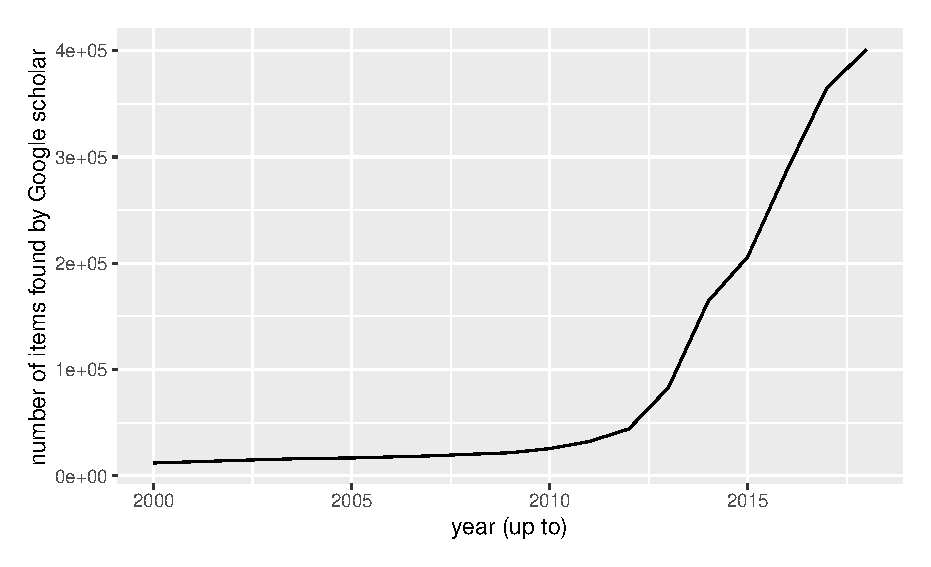
\includegraphics[width=\textwidth]{bigdata.eps}
\end{figure} 
\end{frame}


\begin{frame}{Data structure}
\begin{figure}
\centering
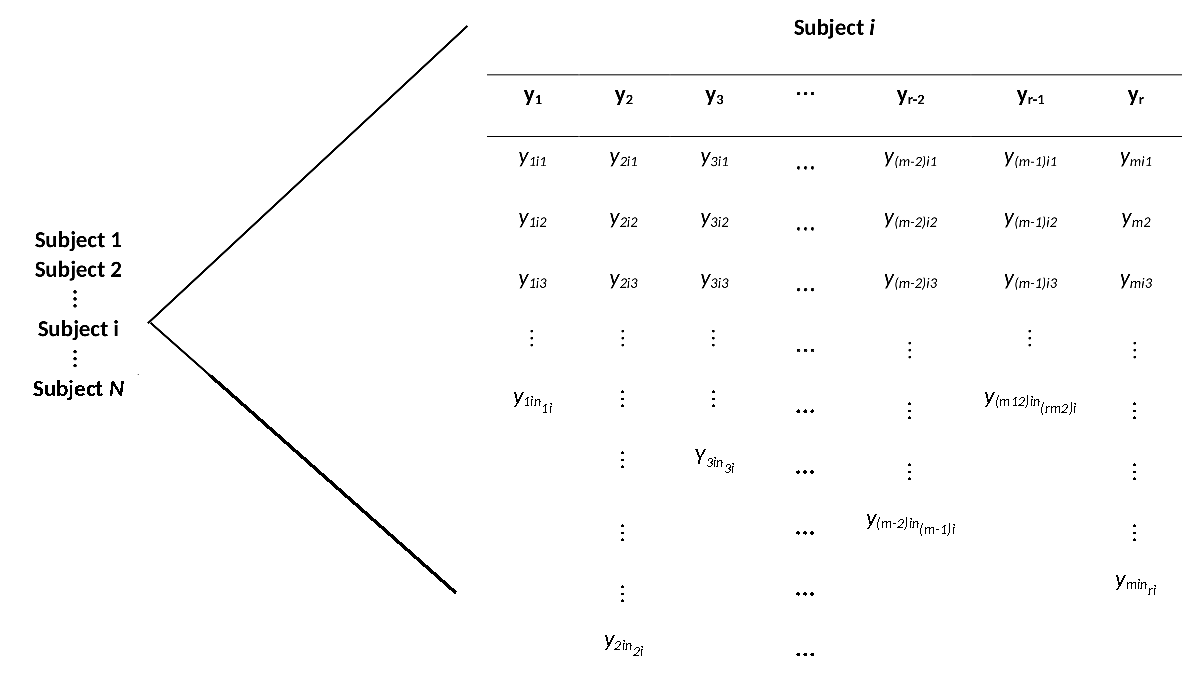
\includegraphics[width=\textwidth]{scheme_new.eps}
\end{figure} 

\end{frame}

\begin{frame}{Clustered big-data}
\begin{itemize}
\item When the sample size, $N$, becomes very large,
\item When the cluster sizes become very large:
\begin{itemize}
\item When the number of measurements per outcome for some clusters, $n_{ri}$'s, becomes very large,
\item When the number of outcomes, $m$, becomes very large.
\end{itemize}
\end{itemize}
\end{frame}

\begin{frame}{Data splitting: a unified approach}

\begin{enumerate}
\item \textbf{Splitting:} split data into smaller chunks in a way that analyzing each of them is easier than the complete data.

\item \textbf{Analyzing}: perform the desired analysis on each split, preferably noting more than the parameter estimates and their covariance matrix should not be required.

\item \textbf{Combining}: the results from several splits should be combined into a single set of results in an appropriate way.

\end{enumerate}

\end{frame}

\begin{frame}{Different types of splitting}

\begin{figure}
\centering
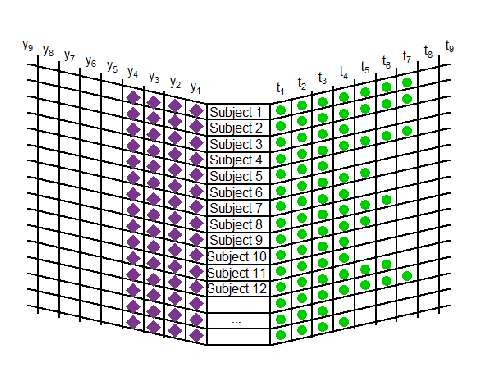
\includegraphics[width=8cm]{long.eps}
\end{figure} 
\end{frame}


\begin{frame}{Random horizontal splitting}

\begin{figure}
\centering
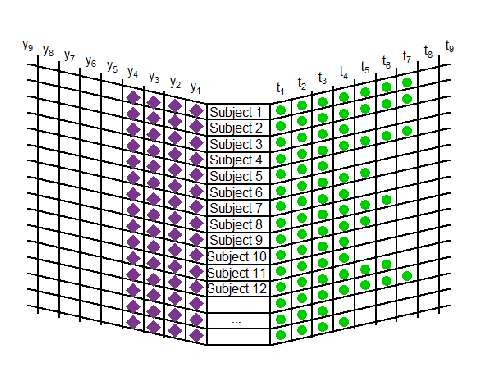
\includegraphics[width=8cm]{long.eps}
\end{figure} 
\end{frame}

\begin{frame}{Structured horizontal splitting}

\begin{figure}
\centering
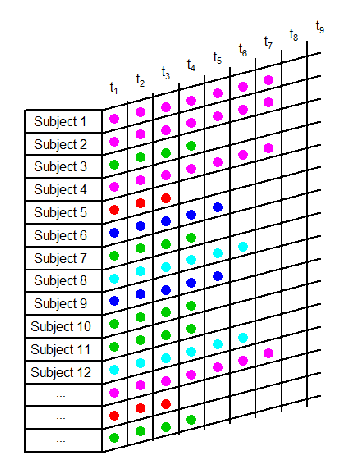
\includegraphics[width=5.5cm]{plot2.eps}
\end{figure} 
\end{frame}

\begin{frame}{How to combine?}

Assume $\widehat{\theta}_1, \ldots, \widehat{\theta}_M$ are the estimated parameters from $M$ sub-samples, the data splitting estimate of this parameter can be computed as follows:
$$\widetilde{\theta} = \sum_{m=1}^M w_m\widehat{\theta_m}.$$
And for the variance:
$$\mathrm{Var}_{horizontal}(\widetilde{\theta}) = \sum_{m=1}^M w_m^2 \sigma_m^2.$$
\end{frame}

\begin{frame}{What about weights?}
\begin{itemize}
\item Equal weights: $w_{equal,i} = \frac{1}{M}$
\item Proportional weights: $w_{prop, i} = \frac{m_i}{N}.$
\item Size proportional weights: $w_{size-prop, i} = \frac{m_i n_i}{\sum_{k=1}^ M m_k n_k}.$
\item Optimal weights: $w_{opt, i} = \frac{1/\sigma^2_i}{\sum_{m=1}^M 1/\sigma^2_m},$
\begin{itemize}
\item as minimizer of $Q = \sum_{m=1}^M w_m^2 \sigma_m^2 - \lambda \left(\sum_{m=1}^M w_m -1 \right).$
\end{itemize}
\end{itemize}
\end{frame}

\begin{frame}{But large clusters...}
\begin{itemize}
\item We have a dataset of book ratings from Amazon.com,
\item each book is rated by different number of people: as small as 1 and
as large as 20,000. \pause
\item Splitting at book level would not help much!
\item But one can split the data within each book.
\end{itemize}

\end{frame}

\begin{frame}{Random vertical splitting}

\begin{itemize}
\item Splitting data within the cluster can be done by sub-sampling:
\begin{itemize}
\item \textbf{Splitting}: a random sub-sample of a reasonable size is taken from each cluster.
\item \textbf{Analysis}: the analysis of interest will be performed on this dataset.
\item \textit{Iterations}: As a new split, a new sub-sample is taken
\item \textbf{Combining}: the same combination rule can be applied on parameter estimates. 
\end{itemize}
\item But the variance is a different story.
\end{itemize}

\end{frame}

\begin{frame}{Variance combination rule for vertical splitting}
$$\mathrm{Var}(\widetilde{\theta}) = W - \left(1 + \frac{1}{M}\right) B,$$

where $W$ and $B$ are within and between sub-samples variances.

$$W = \frac{1}{M} \sum_{i=1}^M \sigma^2_m,\;$$ 
$$B = \frac{1}{M-1} \sum_{i=1}^M \left(\widehat{\theta}_i - \widetilde{\theta} \right)^2.$$

\end{frame}

\begin{frame}{But how many sub-samples?}
\begin{enumerate}
\item \textbf{Start.} Select an initial number of sub-samples, $M_0$, and sub-sampling size $m$. Take $M_0$ sub-samples of size $m$, fit the model to each and obtain $\widehat{\theta}_i$ and its variance $\Sigma_{\widehat{\theta}_i}$ ($i=1,\ldots,M_0$). Then compute 
$$\widetilde{\bftheta}_{M_0} = \sum_{i=1}^{M_0} \widehat{\bftheta}_i,\;\; \Sigma_{\widetilde{\theta_{M_0}}}=\widehat{W}_{M_0} - \left( \frac{M_0+1}{M_0} \right) \widehat{B}_{M_0}.$$
			\item \textbf{Update.} For sub-sampling size $m>M_0$, $m>M_0$, 
$$\widetilde{{\bftheta}}_{m+1}=\frac{m\widetilde{\bftheta}_m + \widehat{\bftheta}_{m+1}}{m+1},$$
$$ \Sigma_{\widetilde{\theta}_{m+1}}=\widehat{W}_{m+1} - \left( \frac{m+1}{m} \right) \widehat{B}_{m+1}.$$
	\item \textbf{Distance.} Compute: $d_{m+1}=d(\widetilde{\bftheta}_{m+1},\widetilde{\bftheta}_{m})$ using an appropriate distance.
	\item \textbf{Stopping rule.} $d_{j} < \varepsilon$ for $j=m+1,\ldots,m+k_0$.
\end{enumerate}
\end{frame}

\begin{frame}{Finite information limit estimators}
\begin{itemize}
\item The amount of information in some clusters is finite
\item In such cases a few sub-samples would be sufficient
\item We have shown in some cases even one or two sub-samples will do the job!
\end{itemize}
\end{frame}


\begin{frame}{Structured vertical splitting?}
\begin{itemize}
\item Vertical splitting based on a pre-defined structure could also be beneficial
\item An important example of this application is modeling several outcomes of interest using random effects.
\end{itemize}
\end{frame}

\begin{frame}{Using random effects to jointly modeling several responses}
\begin{equation*}
\begin{cases}
y_{1ij} = \beta_1 + b_{1i} + \epsilon_{1ij} \\
y_{2ij} = \beta_2 + b_{2i} + \epsilon_{2ij} \\
y_{3ij} = \beta_3 + b_{3i} + \epsilon_{3ij},
\end{cases}
\end{equation*}
we let the three random intercepts to be normally distributed as follows,
\begin{equation*}
\label{eq_SV_D}
\begin{bmatrix}
b_{1i} \\
b_{2i}\\
b_{3i}\\
\end{bmatrix} \sim N \left ( 
\begin{bmatrix}
0 \\
0\\
0\\
\end{bmatrix}, 
D=\begin{bmatrix}
D_{11} & D_{12} & D_{13}\\
 & D_{22} & D_{23}\\
&& D_{33}\\
\end{bmatrix}
\right).
\end{equation*}
Therefore, the parameter of interest, $\bftheta$, is:
\begin{equation*}
\bftheta= (\beta_1,\beta_2,\beta_3, D_{11},D_{22},D_{33},D_{12}, D_{13}, D_{23}).
\end{equation*}
\end{frame}

\begin{frame}{What about more responses?}
\begin{figure}
\centering
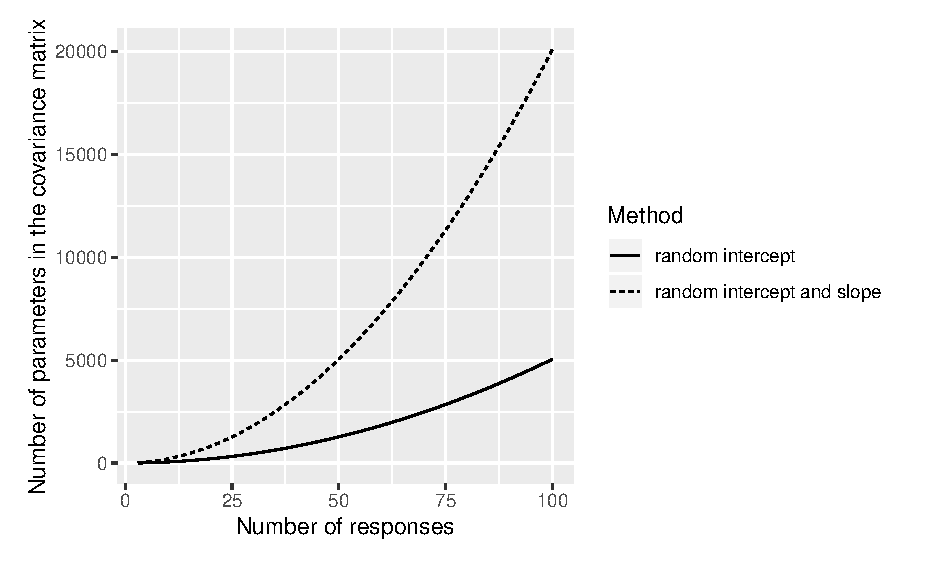
\includegraphics[width=\textwidth]{strucVert.eps}
\end{figure} 


\end{frame}

\begin{frame}{Yes, it is vertical, but where is the structure?}
\begin{figure}
\centering
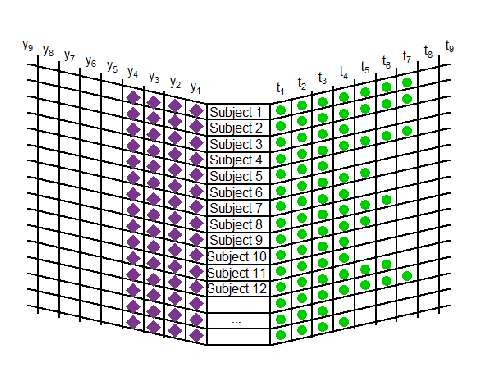
\includegraphics[width=8cm]{long.eps}
\end{figure} 
\end{frame}

\begin{frame}{Back to the example}
\begin{equation*}
\begin{cases}
\bftheta^{(1)}=\theta_{(y_{1ij},y_{2ij})} = (\beta_{1_1},\beta_{2_1},D_{11_1},
,D_{22_1},D_{12_1}) \\
\bftheta^{(2)}=\theta_{(y_{1ij},y_{3ij})} = (\beta_{1_2},\beta_{3_2},D_{11_2},
,D_{33_2},D_{13_2}) \\
\bftheta^{(3)}=\theta_{(y_{2ij},y_{3ij})} = (\beta_{2_3},\beta_{3_3},D_{22_3},
,D_{33_3},D_{23_3}),
\end{cases}
\end{equation*}

\end{frame}

\begin{frame}{Where combination rule fails}

\begin{itemize}
\item A weighted average is a reasonable combination rule both theoretically and intuitively,
\item But it should only be applied on parameter vectors which are each others counterparts.
\item A place where this condition fails is principal component analysis.
\end{itemize}

\end{frame}

\begin{frame}
\begin{itemize}
\item Methods like PCA work based on eigenvalue decomposition of the covariance (or correlation) matrix. 
\item Eigenvalues of a matrix $\Sigma$ can be obtained by solving the following equation,
		$$|\Sigma-\lambda I|,$$ 
\item The first PC is the eigenvector corresponds to the largest eigenvalue.\pause
\item There is no guarantee that these are the same for data from two sub-samples.
\item Think in case of factor analysis where latent underlying factors are there.
\end{itemize}
\end{frame}

\begin{frame}{How to solve the issue}
\begin{itemize}
\item There has been several solutions proposed for this problem:
\begin{itemize}
\item From simple odd methods like averaging the individuals data-points from several sub-samples,
\item to complicated methods like rotating PC's (factor loadings) in a way to make the ones from different sub-samples as similar as possible.
\end{itemize}
\item Our proposed solution was a king of take-the-pencil-instead solution!\pause
\item We proposed to first estimate the covariance matrix based on data-splitting, and then perform PCA on it.
\item We have explored theoretical and practical aspects of this proposal,
\item Also, developed appropriate confidence intervals for the proportion of explained variance.
\end{itemize}
\end{frame}


\begin{frame}{Conclusions}
\begin{itemize}
\item We have developed a unified approach to deal with clustered big data based on data splitting. 
\item Data splitting is similar to methods such as Google's MapReduce, or dplyr's split-apply-combine strategy.
\item The proposed framework makes sure that:
\begin{itemize}
\item While each methodology can deal with one situation, it is easily possible to combine methodologies to deal with a combined situation.

\item The splitting and combining steps of our methodology are as independent as possible from the analyses step, so one can easily (or with a minor modification) use it for its desired analysis.

\end{itemize}
\item R packages {\tt{fastCS}}, {\tt{fastAR1}}, {\tt{fimi}}, {\tt{mifa}}, and {\tt{miscVSS}} are prepared to implemented the methodologies we have developed. They are all publicly and freely available via {\tt{https://github.com/vahidnassiri}}.

\end{itemize}


\end{frame}

\begin{frame}{Immediate future plans}
\begin{itemize}
\item Using developed framework to deal with small data issue.
\item Implementing an R package to perform various currently-implemented-separately methods in a unified fashion. 
\end{itemize}
\end{frame}

\begin{frame}
\begin{figure}
\centering

\includegraphics[width=9cm]{thanks.eps}
\end{figure} 
\end{frame}

\end{document}
